% !TEX program = xelatex
\documentclass{article}
\usepackage[margin=1in]{geometry}
\usepackage{nopageno} % no page numbers

\usepackage{graphicx}
\graphicspath{ {./graphics/} }
\usepackage[dvipsnames]{xcolor}
\definecolor{CrispBlue}{HTML}{0176AE}

\usepackage{fontspec}
\usepackage{tcolorbox}
\usepackage{etoolbox}
\BeforeBeginEnvironment{verbatim*}{\begin{tcolorbox}[colback=CrispBlue!5!white,colframe=CrispBlue!75!black]}%
\AfterEndEnvironment{verbatim*}{\end{tcolorbox}}%


\usepackage{hyperref}
\hypersetup{
    colorlinks,
    citecolor=black,
    filecolor=black,
    linkcolor=black,
    urlcolor=black
}

\usepackage{subcaption}
\setlength{\parindent}{0pt}
\setlength{\parskip}{1em}

\usepackage{tocloft}
\renewcommand{\cftpartleader}{\cftdotfill{\cftdotsep}}
\renewcommand{\cftsecleader}{\cftdotfill{\cftdotsep}}

\usepackage{fancyhdr}
\pagestyle{fancy}
\fancyhf{}
\lhead{ECE 530: Cloud Computing}
\rhead{Homework \#3}
\rfoot{Page \thepage}

\renewcommand{\listfigurename}{List of Figures}

\begin{document}
\setmainfont{SF Pro Text}
\setsansfont{SF Pro Text}
\setmonofont{SF Mono}
\renewcommand{\familydefault}{\sfdefault}

\thispagestyle{empty}
\begin{titlepage}
\vspace*{\fill}
\begin{center}
\textsc{\Huge{ECE 530: Cloud Computing}}\\[3em]
\textsc{\LARGE Homework \#3: Linux Containers}\\[6em]
\textsc{\Large\hspace{2em} Amber Disher -- 101839171 -- adisher1@unm.edu\\[0.8em]
Marshall Hundemer -- 101736010 -- mhundemer@unm.edu\\[1em]
\hspace{3.5em} David Kirby -- 101652098 -- davidkirby@unm.edu}\\[3em]
\textsc{\Large Spring 2021}
\end{center}
\vfill
\begin{figure}[h]
\begin{subfigure}{0.5\textwidth}

\includegraphics[width=0.5\linewidth]{Docker.png}
\end{subfigure}
\begin{subfigure}{0.6\textwidth}\hspace{1em}

\includegraphics[width=0.8\linewidth]{new-soe-logo.png}
\end{subfigure}
\end{figure}
\end{titlepage}
\setcounter{figure}{0}

\tableofcontents

\addcontentsline{toc}{section}{1\ \ \ \ List of Figures}
\listoffigures
\newpage
\setcounter{section}{+1}

\hypersetup{
    linkcolor=CrispBlue,
    urlcolor=CrispBlue,
    breaklinks=true
}
\section{Abstract}
Docker is a platform to easily maintain highly configurable instances. It can be set up and ran in milliseconds, and can create globally accessible services. For homework \#3 we were tasked to create a Dockerfile that can build images automatically, then to deploy a distributed database based on Linux containers. Our deployment must contain at least two containers and therefore at least two database instances. The instances must be connected to each other and contain part of the data.


\section{Introduction}
For our deployment we chose MongoDB, a document-oriented NoSQL database. To create our images we used the Dockerfile shown in the \nameref{sec:Appendix}. We quickly learned that Dockerfiles are limited in their build capabilities, notably with creating networks and creating multiple images at once. These issues can be solved using docker-compose, but that is beyond the scope of this assignment.






\section{Deployment}
In order to use Docker, we needed to install the necessary software. For reference, our host machine is running macOS Big Sur on an Apple silicon-based MacBook Air. We installed Docker using Homebrew, a package manager for macOS, and needed to run the latest Docker version in order to work on ARM processors. One of the most important features of Docker allows us to build on ARM, but then deploy on other architectures as well.

\begin{tcolorbox}[colback=CrispBlue!5!white,colframe=CrispBlue!75!black,title=Install Docker via Homebrew]
\begin{verbatim}
    brew install docker
\end{verbatim}
\end{tcolorbox}

\begin{tcolorbox}[colback=CrispBlue!5!white,colframe=CrispBlue!75!black,title=Docker verification]
\begin{verbatim}
# Verify Docker version

    docker -v

# Check Docker images

    docker images
\end{verbatim}
\end{tcolorbox}

\begin{tcolorbox}[colback=CrispBlue!5!white,colframe=CrispBlue!75!black,title=Pulls latest version of MongoDB from Docker Hub]
    \begin{verbatim}    
    docker pull mongo
\end{verbatim}
\end{tcolorbox}
The output of these commands is shown in \autoref{fig:Docker-verify}.

\begin{figure}[ht]
    \centering
    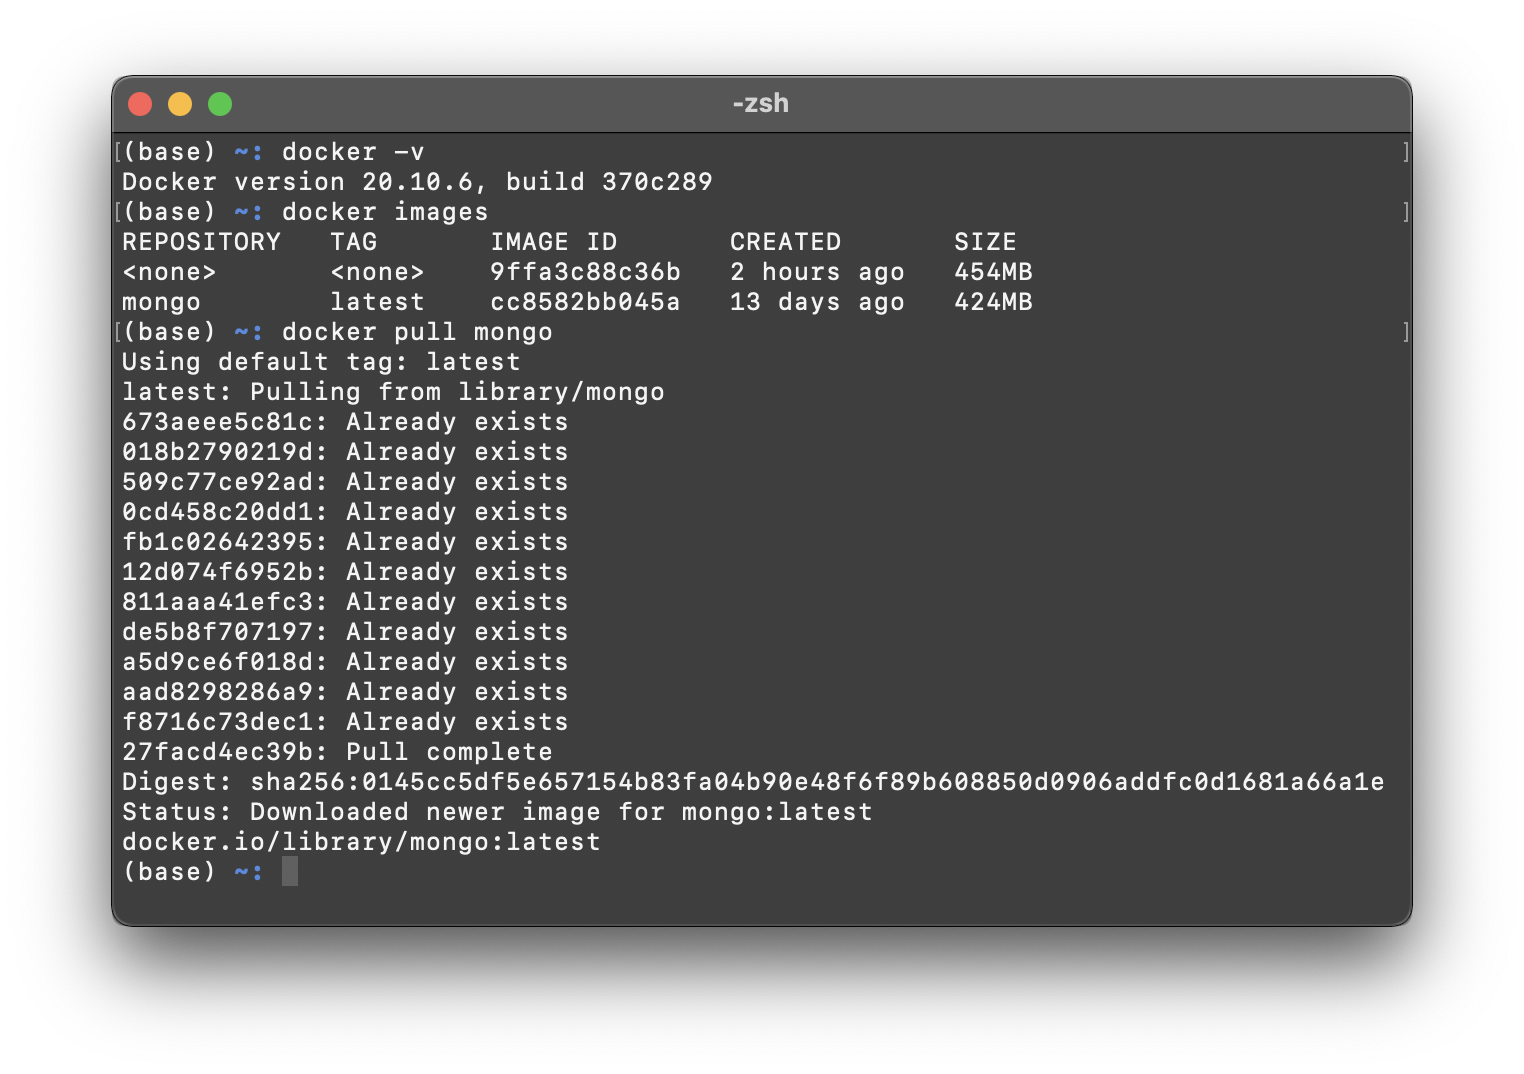
\includegraphics[width=0.99\textwidth]{Docker-verify.png}
    \vspace{-3em}\caption{Verification of Docker Installation.}
    \label{fig:Docker-verify}
\end{figure}

\newpage
Once Docker was installed we needed to set up a network to which our databases could join. Docker has default networks installed:
\begin{itemize}
    \item host -- For standalone containers, removes network isolation between the container and the Docker host, and uses the host’s networking directly.
    \item bridge -- The default network driver. Bridge networks are usually used when your applications run in standalone containers that need to communicate.
\end{itemize}

The default bridge network allow us to configure the network, but all the containers use the same settings, such as MTU and iptables rules. In addition, configuring the default bridge network happens outside of Docker itself, and requires a restart of Docker. Creating our own bridge network, created and configured using \texttt{docker network create}, allows different groups of applications to have different network requirements, allows us to configure each user-defined bridge separately. Containers connected to the same user-defined bridge network effectively expose all ports to each other.

\begin{tcolorbox}[colback=CrispBlue!5!white,colframe=CrispBlue!75!black,title=List all networks created in Docker]
\begin{verbatim}    
docker network ls
\end{verbatim}
\end{tcolorbox}

\begin{tcolorbox}[colback=CrispBlue!5!white,colframe=CrispBlue!75!black,title=Create our user-defined network]
\begin{verbatim}
docker network create mongo-net
\end{verbatim}
\end{tcolorbox}

\begin{figure}[ht]
    \centering
    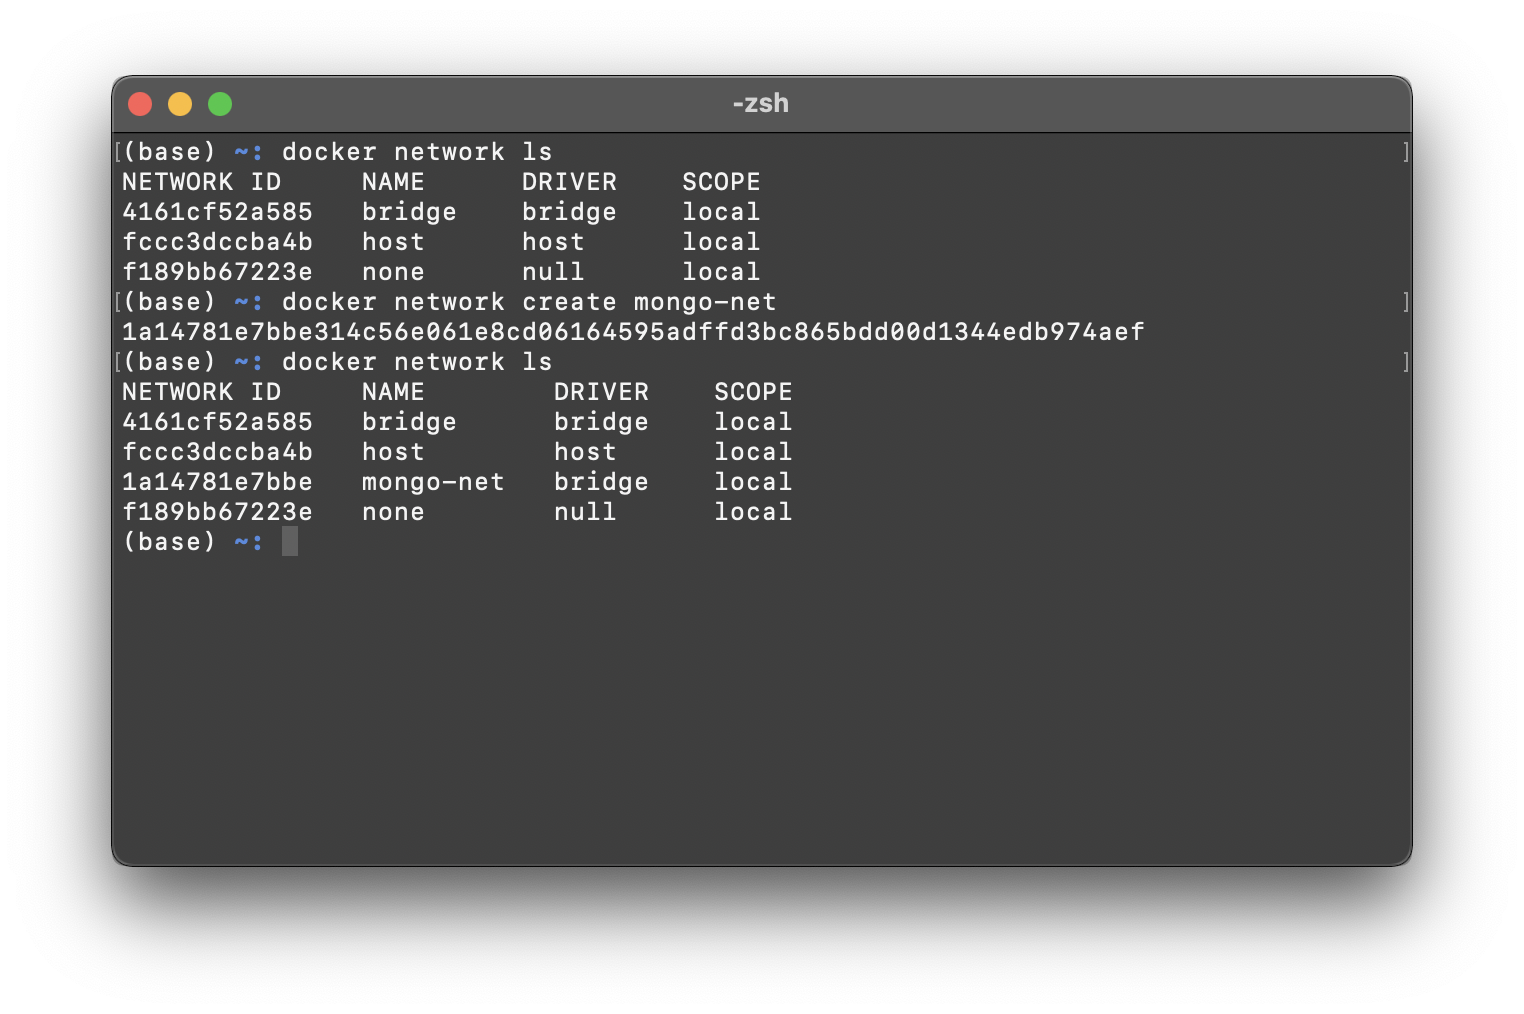
\includegraphics[width=0.99\textwidth]{Docker-network.png}
    \vspace{-3em}\caption{Creation of User-defined Network.}
    \label{fig:Docker-network}
\end{figure}

\newpage
Now that our network was created (see \autoref{fig:Docker-network}), we began creating our containers from the Mongo image and connecting them altogether.

\begin{tcolorbox}[colback=CrispBlue!5!white,colframe=CrispBlue!75!black,title=Create first MongoDB image]    
\begin{verbatim}
docker run -p 30001:27017 --name mongo1 --net mongo-net mongo \
mongod --replSet mongo-set
\end{verbatim}
\end{tcolorbox}

\begin{itemize}
    \item \verb|docker run| -- Start a container from an image
    \item \verb|-p 30001:27017| -- Expose port 27017 in our container, as port 30001 on the localhost
    \item \verb|--name mongo1| -- Name this container ``mongo1''
    \item \verb|--net mongo-net| -- Add this container to the ``mongo-net'' network.
    \item \verb|mongo| -- the name of the image we are using to spawn this container
    \item \verb|mongod --replSet mongo-set| -- Run mongod while adding this mongod instance to the replica set named ``mongo-set''
\end{itemize}

\newpage
We can see in \autoref{fig:Docker-Ubuntu} that we are running Ubuntu 18.04.5 LTS and MongoDB 4.4.5 on aarch64 (ARM) architecture.

\begin{figure}[h!]
    \centering
    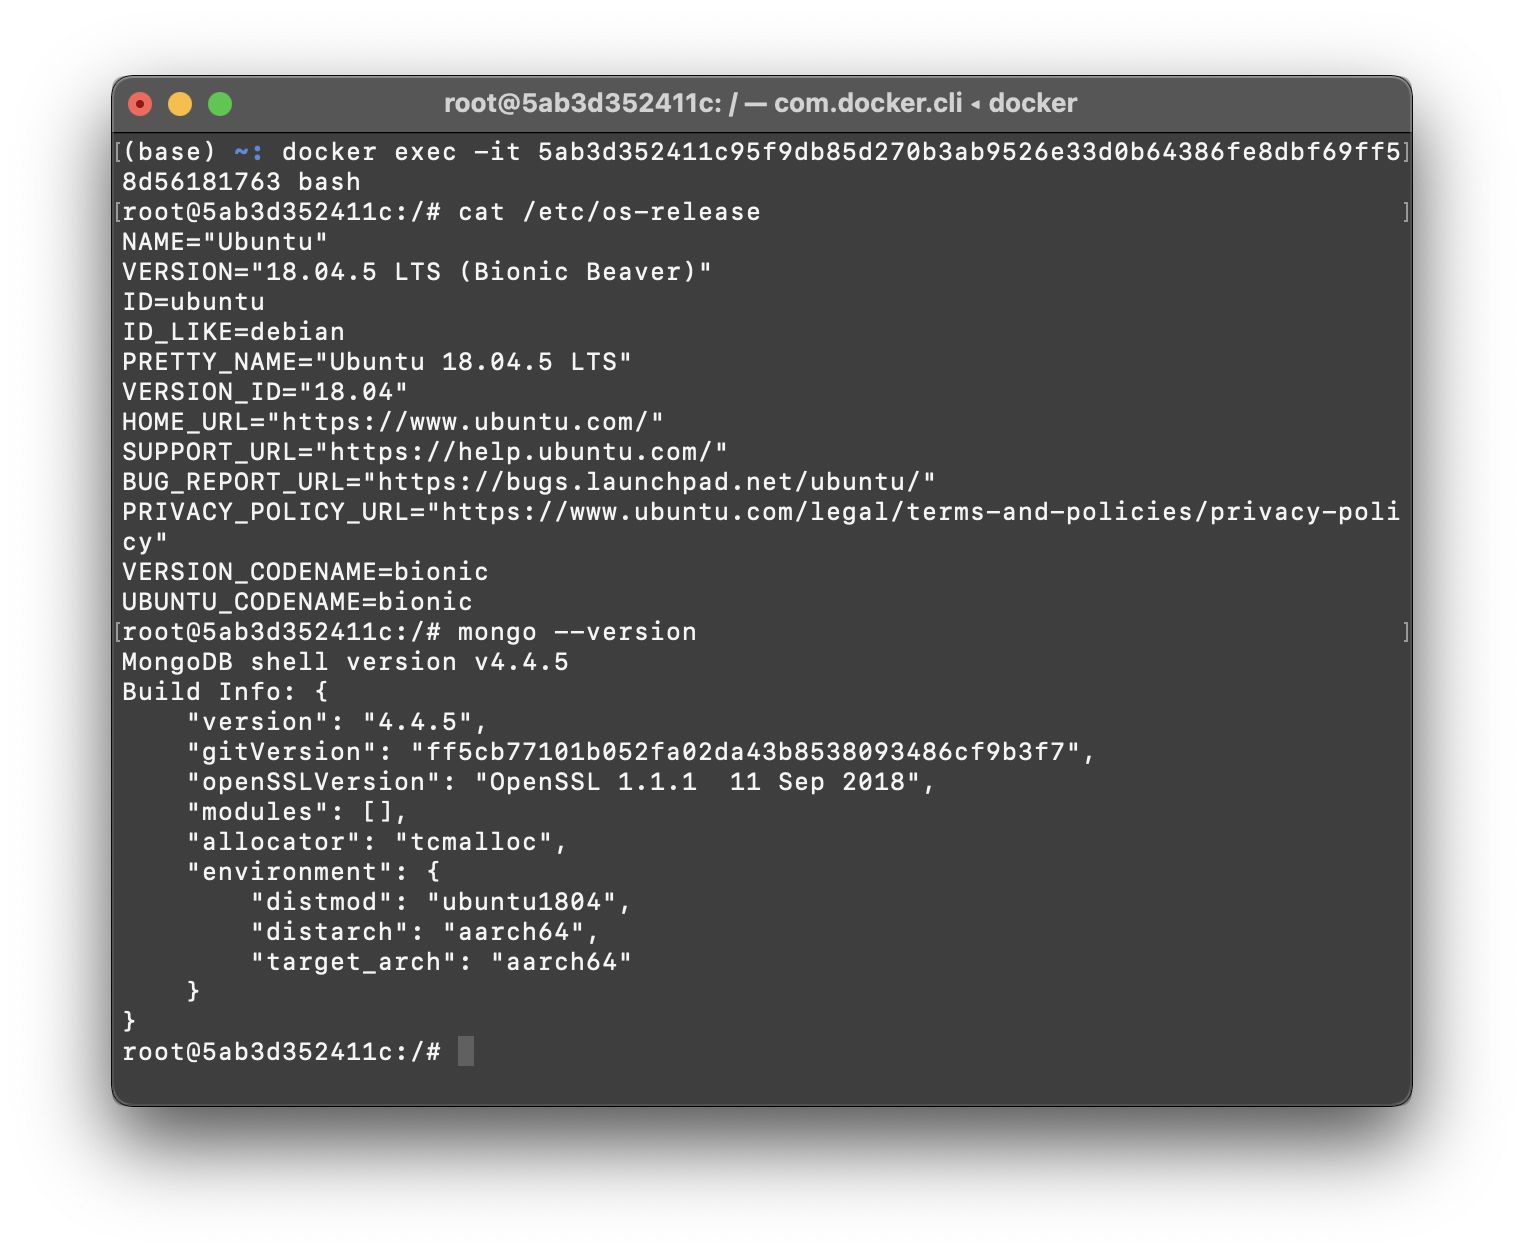
\includegraphics[width=0.99\textwidth]{Docker-Ubuntu.png}
    \vspace{-3em}\caption{Ubuntu and MongoDB Version Checks.}
    \label{fig:Docker-Ubuntu}
\end{figure}

We then created the secondary images, each of which needed to be run in a separate terminal tab, and finally after all database containers were created, we turned them into a replica set.

\begin{tcolorbox}[colback=CrispBlue!5!white,colframe=CrispBlue!75!black,title=Create secondary MongoDB images]    
\begin{verbatim}    
docker run -p 30002:27017 --name mongo2 --net mongo-net mongo \
mongod --replSet mongo-set

docker run -p 30003:27017 --name mongo3 --net mongo-net mongo \
mongod --replSet mongo-set
\end{verbatim}
\end{tcolorbox}

\newpage

We started our Docker container directly into our MongoDB and began configuring the connections.
\begin{tcolorbox}[colback=CrispBlue!5!white,colframe=CrispBlue!75!black,title=Connect to \texttt{mongo1} and configure it to be the primary]
\begin{verbatim}
docker exec -it mongo1 mongo

> db = (new Mongo('localhost:27017')).getDB('test')

> config = {
  	"_id" : "mongo-set",
  	"members" : [
  		{
  		    "_id" : 0,
  		    "host" : "mongo1:27017"
  		},
  		{
  		    "_id" : 1,
  		    "host" : "mongo2:27017"
  		},
  		{
  		    "_id" : 2,
  		    "host" : "mongo3:27017"
  		}
  	]
  }
\end{verbatim}
\end{tcolorbox}

The results of the above commands are shown in \autoref{fig:Docker-DB}. Then we initiated the configuration file we just created and received confirmation by noticing the change in command prompt.

\begin{tcolorbox}[colback=CrispBlue!5!white,colframe=CrispBlue!75!black,title=Initiate our replica set using our just created config file]
\begin{verbatim}
> rs.initiate(config)

mongo-set:PRIMARY> # Confirms that we are on PRIMARY DB
\end{verbatim}
\end{tcolorbox}

We then wrote data to our primary DB to verify it (see \autoref{fig:Docker-Write-Read}), writing a document ``ECE530''. It is important to note that data can only be written to the primary DB, but, as we will show later, can be read from any of the databases. If for some reason the primary database goes down, one of the others will become primary and allow for robustness.

\begin{tcolorbox}[colback=CrispBlue!5!white,colframe=CrispBlue!75!black,title=Write data to \texttt{mongo1} -- our primary DB and then read it]
\begin{verbatim}
> db.mycollection.insert({name : 'ECE530'})

> db.mycollection.find()
\end{verbatim}
\end{tcolorbox}


\begin{figure}[h!]
    \centering
    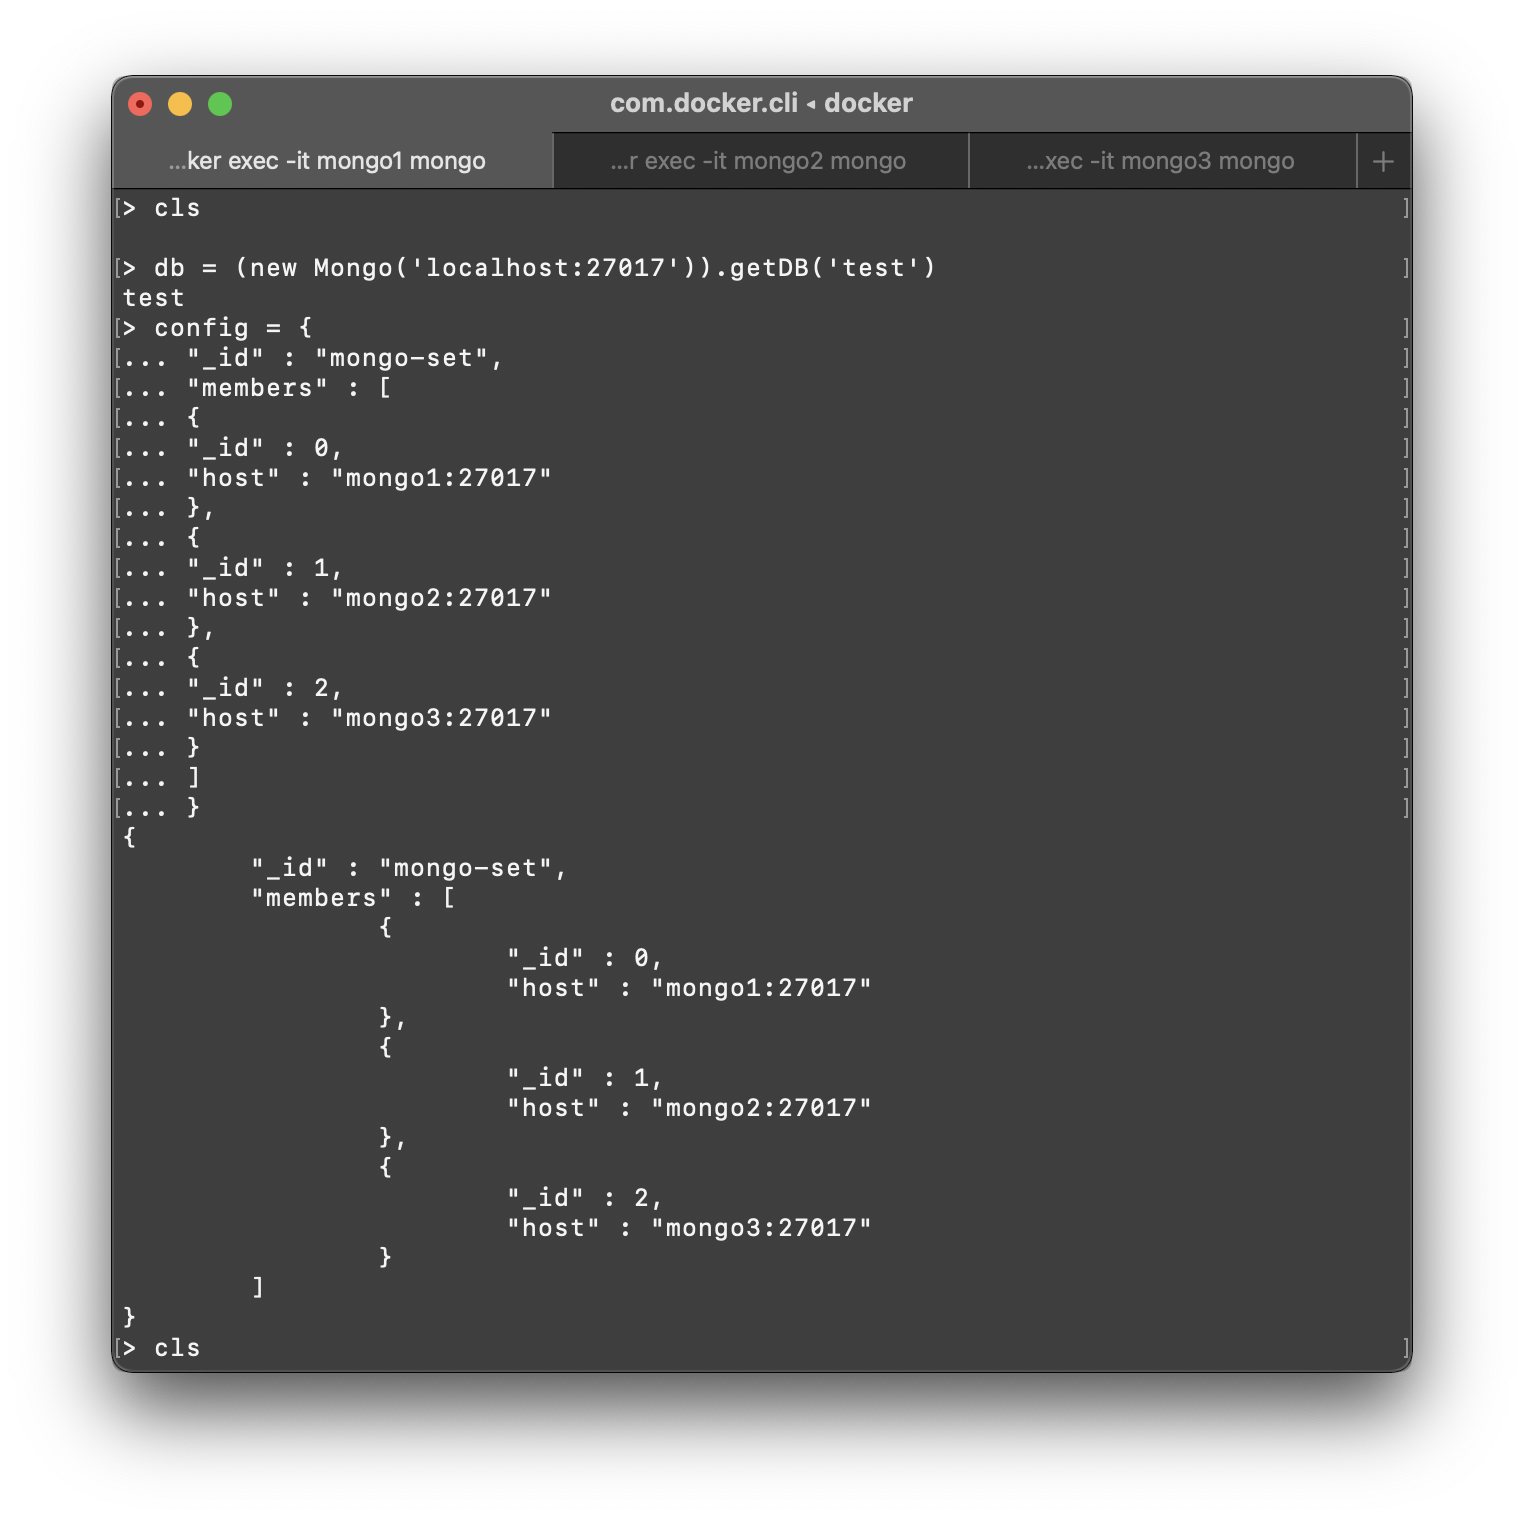
\includegraphics[width=0.99\textwidth]{Docker-DB.png}
    \vspace{-3em}\caption{Database Connection and Configuration.}
    \label{fig:Docker-DB}
\end{figure}

\newpage
We then connect to each of our secondary databases and test to see if our document gets replicated there as well.

\begin{tcolorbox}[colback=CrispBlue!5!white,colframe=CrispBlue!75!black,title=Test that data is being replicated to \texttt{mongo2} and \texttt{mongo3} respectively]
\begin{verbatim}
> db2 = (new Mongo('mongo2:27017')).getDB('test')

> db2.setSecondaryOk()

> db2.mycollection.find()



> db3 = (new Mongo('mongo3:27017')).getDB('test')

> db3.setSecondaryOk()

> db3.mycollection.find()
\end{verbatim}
\end{tcolorbox}

\begin{figure}[ht]
    \centering
    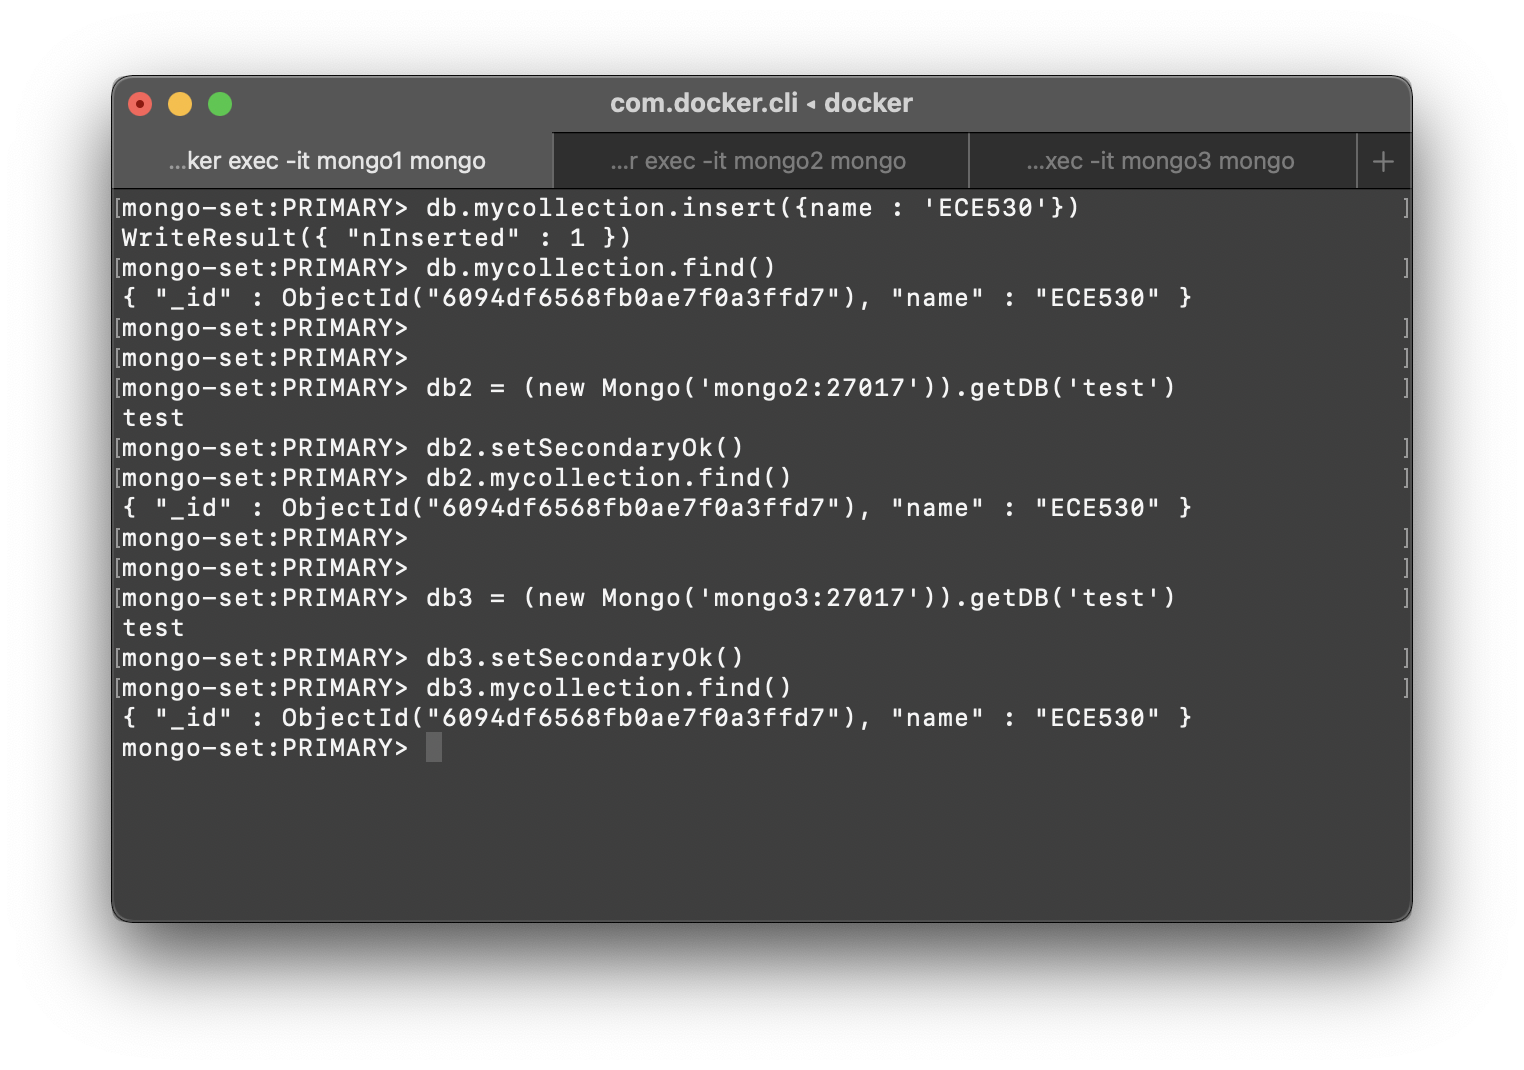
\includegraphics[width=0.99\textwidth]{Docker-Write-Read.png}
    \vspace{-3em}\caption{Database Write, Read, and Replication.}
    \label{fig:Docker-Write-Read}
\end{figure}

\section{Conclusion}
In conclusion, we were successful in creating a Dockerfile to create images of MongoDB, although we found Dockerfiles limited. We set up a  user-defined network for our databases, created three MongoDB databases from our Docker image, and designed those databases to be a replica set. We tested writing data to our primary database and confirmed that the data is indeed distributed. For future work, we would like to explore docker-compose to attempt automating this entire process.

\section{Extra}
While Docker makes configuring and accessing containers extremely easy using the command line interface, it is also very helpful to view our images and containers using a graphical user interface. For example, we show our created replica set in both the Docker Desktop (\autoref{fig:Docker-Desktop}) and in Visual Studio Code, which has built-in Docker support. Using VSCode, we can even view files within Ubuntu image (\autoref{fig:Docker-VSCode}), view all of our containers, images, networks, volumes, and much more at a glance, and even start, stop, and remove items.


\begin{figure}[ht]
    \centering
    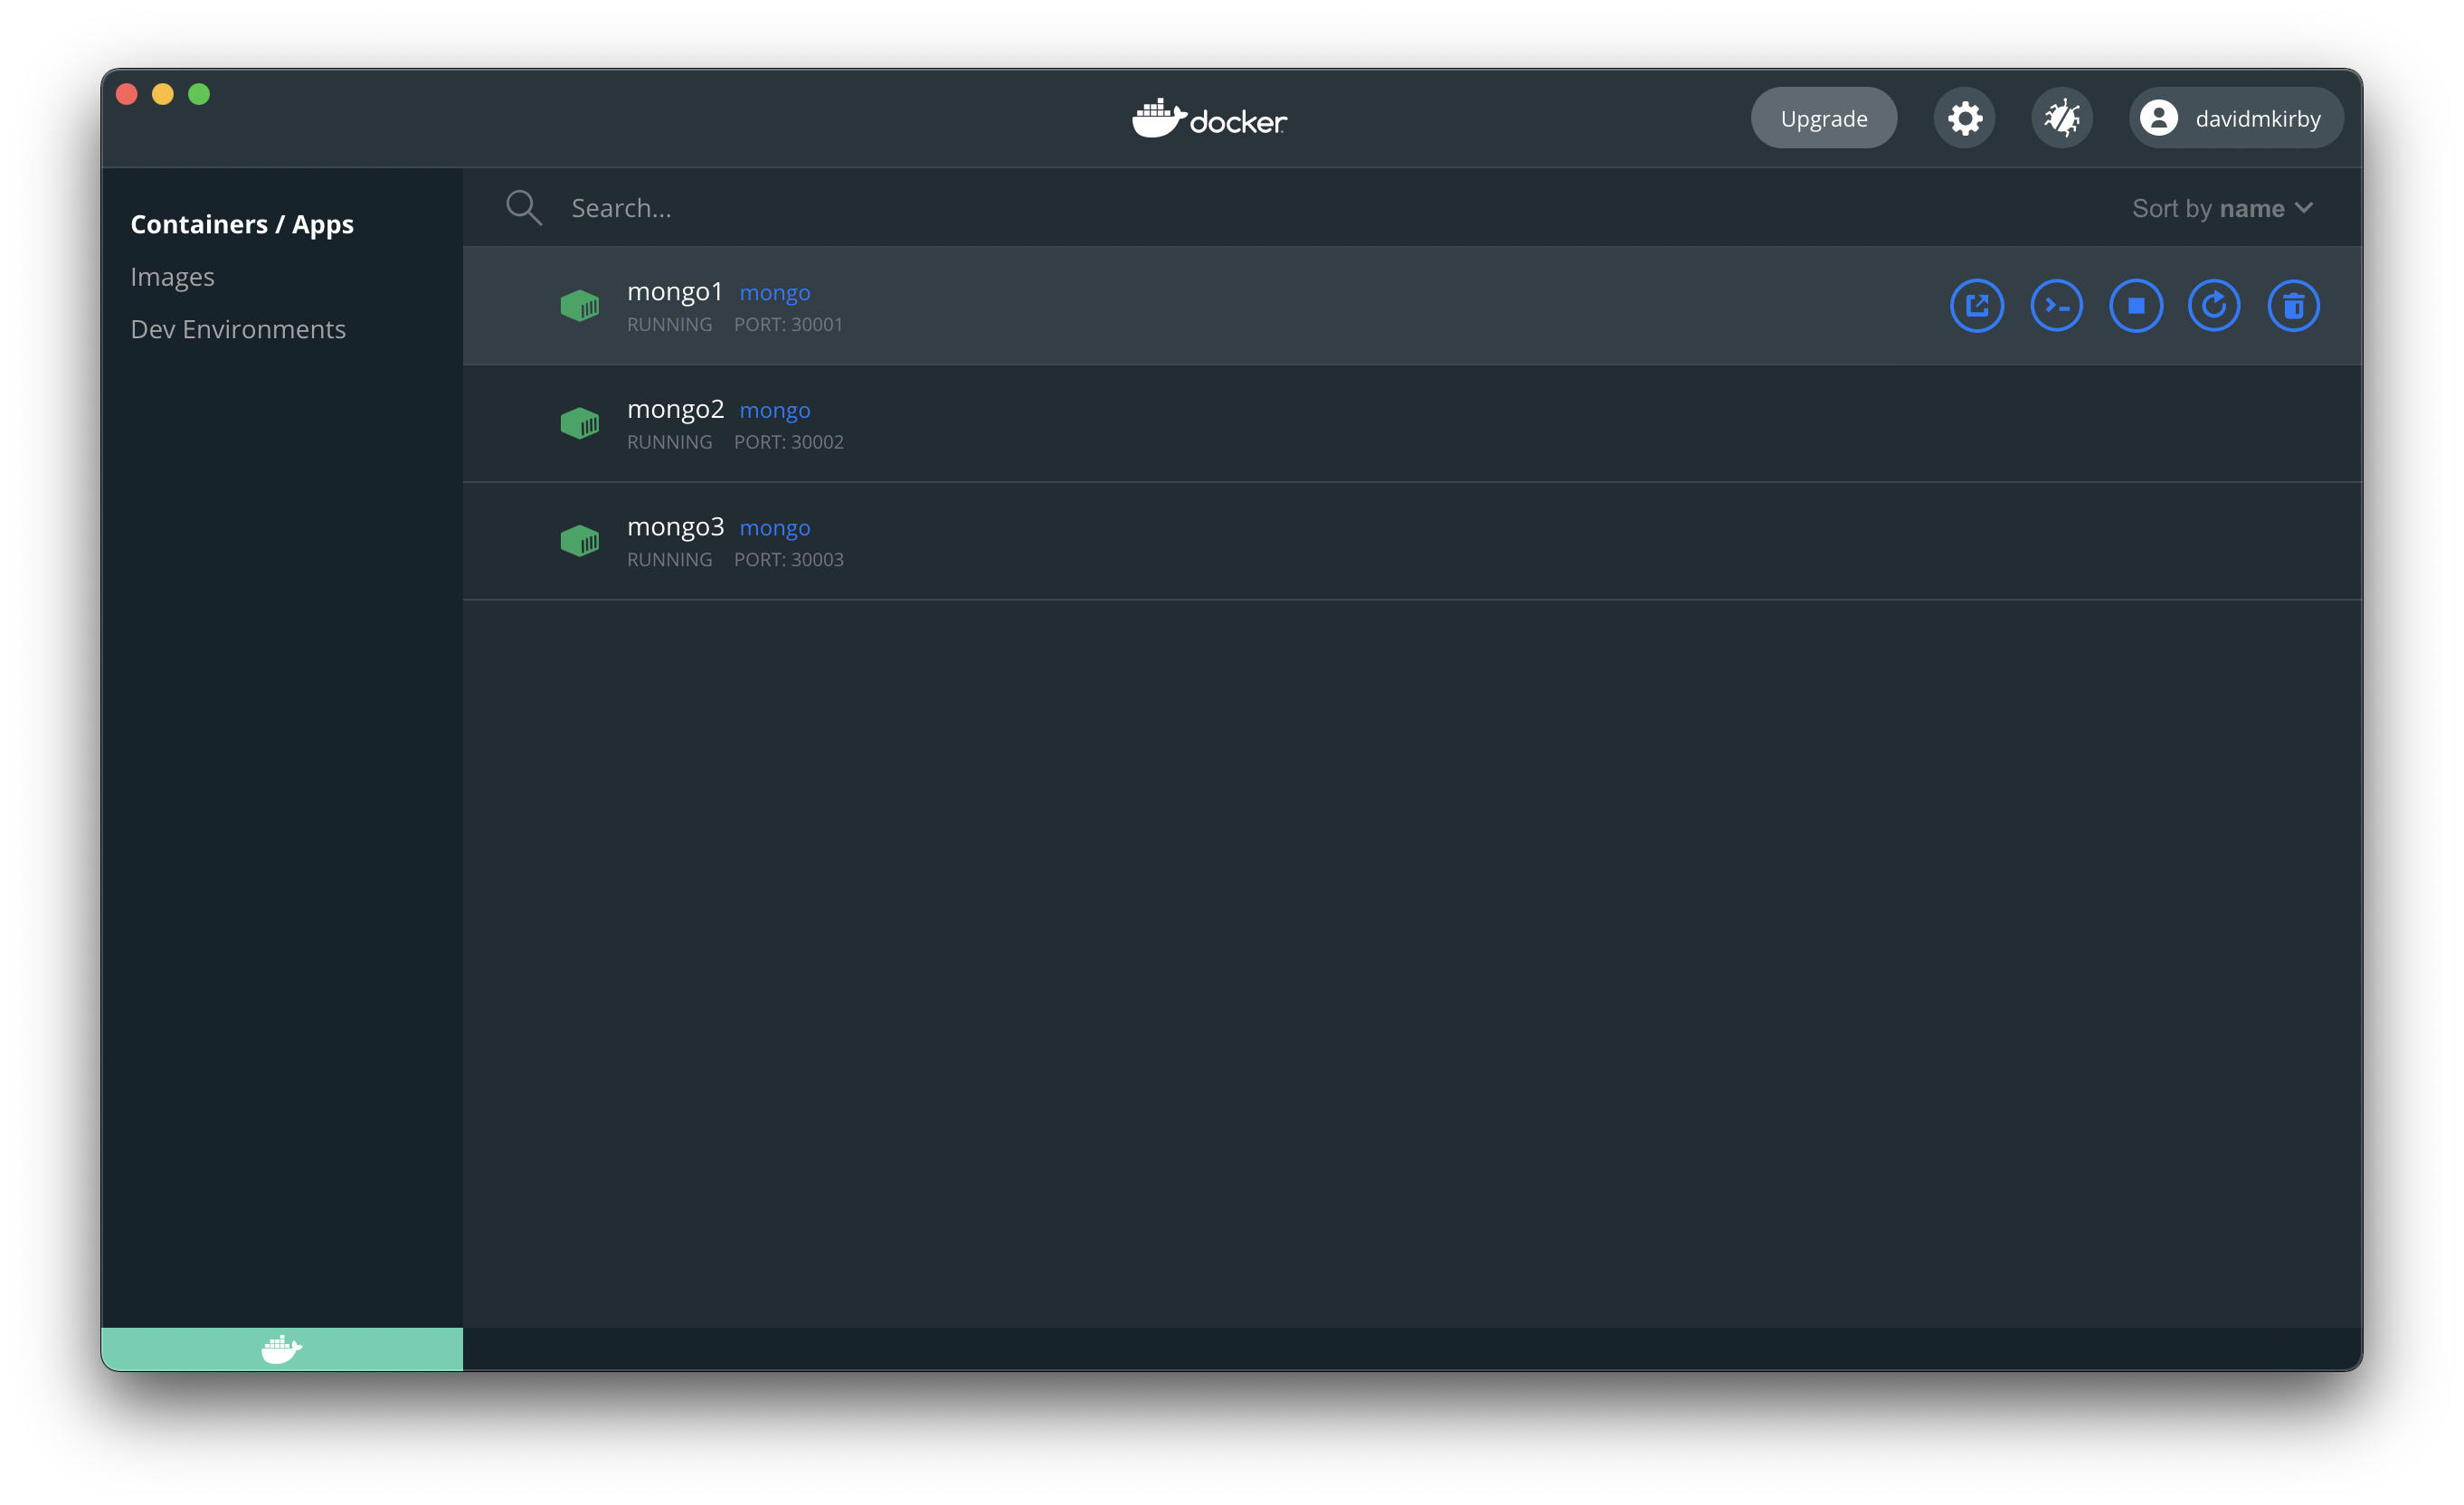
\includegraphics[width=0.96\textwidth]{Docker-Desktop.png}
    \vspace{-1em}\caption{Docker Desktop.}
    \label{fig:Docker-Desktop}
\end{figure}

\begin{figure}[ht]
    \centering
    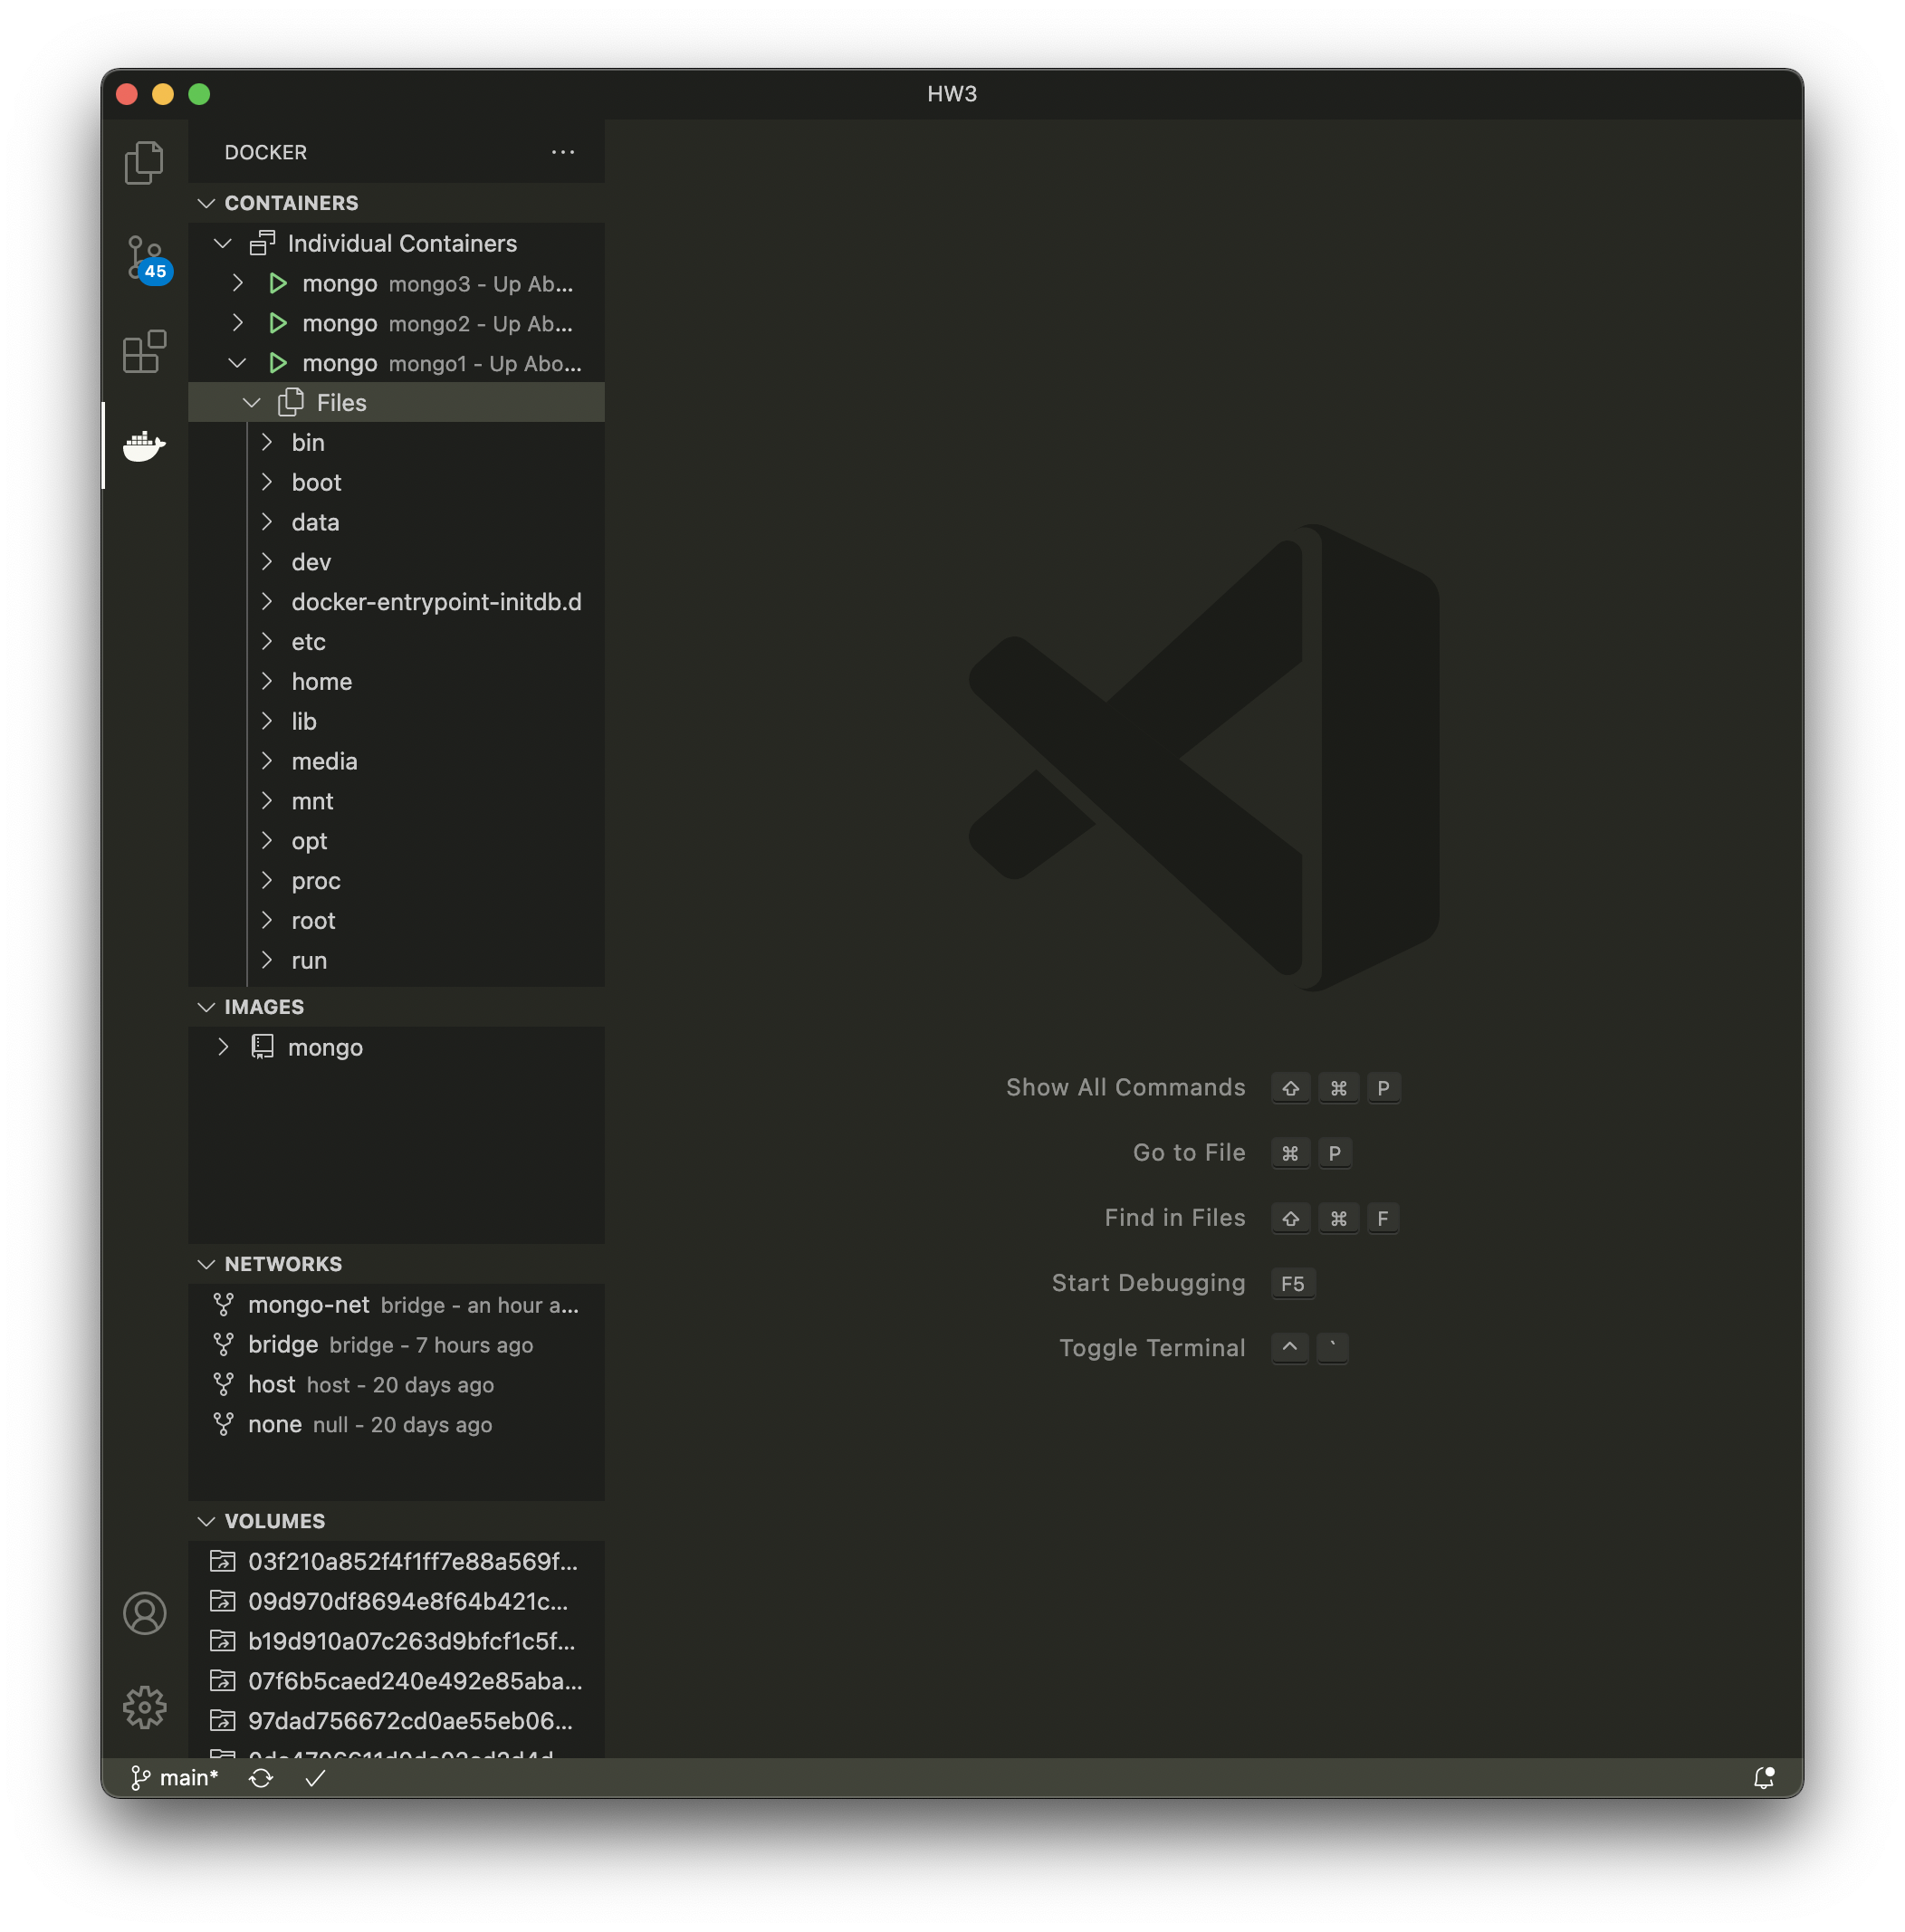
\includegraphics[width=0.99\textwidth]{Docker-VSCode.png}
    \vspace{-2em}\caption{Microsoft Visual Studio Code Docker Support.}
    \label{fig:Docker-VSCode}
\end{figure}








\section{Appendix}\label{sec:Appendix}

\begin{tcolorbox}[colback=CrispBlue!5!white,colframe=CrispBlue!75!black,title=Dockerfile]
\begin{verbatim}
# Pulls latest version of MongoDB from Docker Hub

    FROM mongo
    LABEL maintainer=davidkirby@unm.edu

# Automatically update Ubuntu

    RUN apt-get update && apt-get install -y

# Open Port for MongoDB to connect to host

    EXPOSE 27017
\end{verbatim}
\end{tcolorbox}
\end{document}